\documentclass[]{article}

\usepackage[utf8]{inputenc}
\usepackage{array}
\usepackage{wrapfig}
\usepackage{multirow}
\usepackage{tabu}
\usepackage{graphicx}
\usepackage{amsmath,mathtools}
\newcommand{\code}[1]{\texttt{#1}}

\usepackage{geometry}
 \geometry{
letterpaper,
 total={215mm,279mm},
 left=45mm,
 right=45mm,
 top=25mm,
tmargin = 15mm,
 bottom=25mm,
 }


\begin{document}

\title{Homework 1}
\author{Joshua Michalenko\\ ELEC 677: Deep Learning \\  Dr. Ankit Patel}
\date{10/04/16}
\maketitle



\section{Problem 1: Backpropogation in a simple Nueral Network}
\subsection{Part A:  Dataset}

The plot of the Two Moons dataset is displayed in Figure \ref{fig:partA}

\begin{figure}[ht]
        \centering
        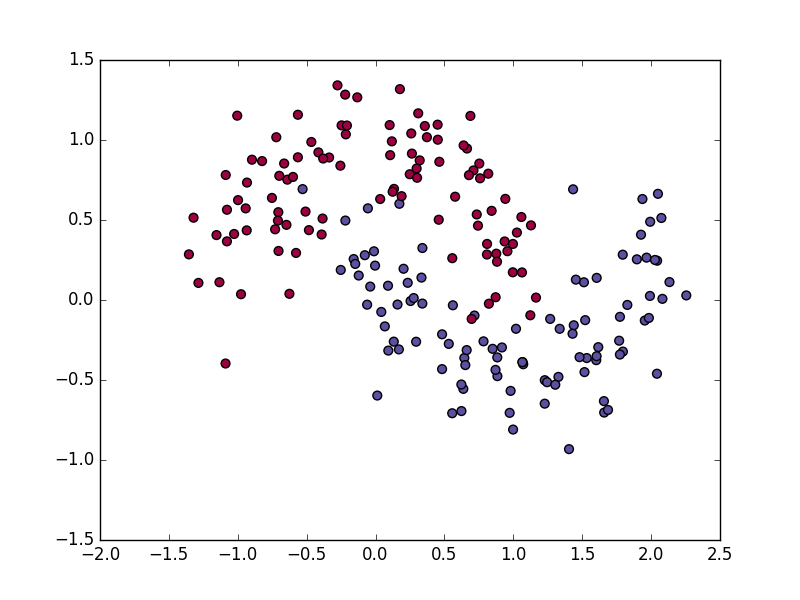
\includegraphics[width=10cm]{figures/twoMoons.png}

 	\caption{Two moons dataset displayed in matplotlib}

 	 \label{fig:partA}
\end{figure}


\subsection{Part B - Activation Functions}
\subsubsection{Part B1 - Derive the derivative for sigmoid function}
\begin{align*} 
\sigma(z)= f(z) = \frac{1}{1+e^{-z}}  &= (1+ e^{-z})^{-1} \\
\frac{df}{dz} : = -1* (1+ e^{-z})^{-2} * -e^{-z}  &= e^{-z}(1+ e^{-z})^{-2}  \text{~~~(by chain rule)}\\
 &= \frac{e^{-z}}{(1+ e^{-z})^{2}  } \\
 &= \frac{1-e^{-z}+1}{(1+ e^{-z})^{2}  }\text{  ~~~(add and subtract a 1)} \\
 &= \frac{1+e^{-z}}{(1+ e^{-z})^{2} } -  \frac{1}{(1+ e^{-z})^{2} }  \text{  ~~~(split terms)}\\
 &= \frac{1}{1+ e^{-z} } -  \frac{1}{(1+ e^{-z})^{2} }  \\
 &= \sigma(z) -  \frac{1}{(1+ e^{-z})^{2} }  \\
 &= \sigma(z) -  \left ( \frac{1}{(1+ e^{-z}) } \right )^2  \\
 &= \sigma(z) -  \sigma(z)^2  \\
\Aboxed{f'(z) &= \sigma(z) (1-  \sigma(z)) } \\
\end{align*}

\subsubsection{Part B2 - Derivative for Tanh function}

\begin{align*} 
f(z) = \text{tanh}(z) &= \frac{\text{sinh}(z)}{\text{cosh}(z)} \\
&= \frac{e^z - e^{-z}}{e^z + e^{-z}} \\
\frac{df}{dz} : &=  \frac{\text{cosh}(z) * \text{sinh}'(z) -  \text{sinh}(z)  * \text{cosh}'(z)}{(\text{cosh}(z))^2}  \text{~~~(by quotient rule)} \\ 
&=  \frac{\text{cosh}(z)^2 1  \text{sinh}(z)^2 }{(\text{cosh}(z))^2} \\ 
&=  \frac{\text{cosh}(z)^2}{\text{cosh}(z)^2} - \frac{\text{sinh}(z)^2}{\text{cosh}(z)^2}\\ 
\Aboxed{f'(z) &= 1- \text{tanh}^2(z)}\\ 
\end{align*}


\subsubsection{Part B3 - Derivative for ReLu function}


\end{document}